Artificial neural networks (ANN) first appeared as a novel way of solving problems that was inspired by the way the brain computes. Generations of neural networks can be classified by their basic compute unit, the neuron model. Under this scheme, the \textbf{first generation} used \textsc{on-off} threshold gates, also known as perceptrons. The basic functionality is that if the input value is above a certain threshold, the neuron will output a 1 and 0 otherwise. These type of network is limited to binary outputs. First generation ANN are able to compute every boolean function using a single hidden layer~\cite{third-gen-nn-Maass1997}.

The \textbf{second generation} of neural models make use of an activation function which enables the output of analog values. The typical activation function is a sigmoid (eq. \ref{eq:neuro:sigmoid}). Whenever the activation function reaches a certain threshold, the neuron will be ``fire''.

\begin{equation}
  \sigma(x) = \frac{1}{1 + e^{-x}}
  \label{eq:neuro:sigmoid}
\end{equation}

A notable addition is that multi-layered network of the second generation are able to be trained using gradient descent-based algorithms~\cite{hecht1989-backprop-theory}. One drawback is that they are not biologically plausible, for they can be interpreted as neurons using rate coding which is an unlikely candidate for fast computations in the brain~\cite{third-gen-nn-Maass1997}.

Spiking neural networks are considered the \textbf{third generation} of ANN, the main difference is that their activation function is closer to the one observed in biological neurons. Some neuron models used were described in previous sections. Third generation ANN are able to approximate any analog continuous function~\cite{third-gen-nn-Maass1997}. 
%\begin{figure}
%  \begin{center}
%    \begin{subfigure}{0.25\textwidth}
%      %    \vspace*{0.8em}
%      \centering
%      \captionsetup{justification=centering}
%      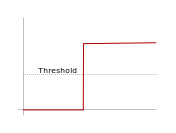
\includegraphics[width=\textwidth]{perceptron}
%      \caption{Perceptron}
%      \label{fig:neuro:perceptron}
%    \end{subfigure}
%    \begin{subfigure}{0.25\textwidth}
%      %    \vspace*{0.8em}
%      \centering
%      \captionsetup{justification=centering}
%      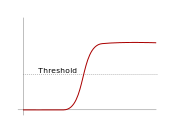
\includegraphics[width=\textwidth]{sigmoid}
%      \caption{Sigmoid}
%      \label{fig:neuro:sigmoid}
%    \end{subfigure}
%    \begin{subfigure}{0.265\textwidth}
%      \centering
%      \captionsetup{justification=centering}
%      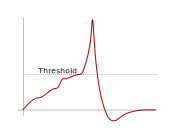
\includegraphics[width=\textwidth]{spike}
%      \caption{Spike}
%      \label{fig:neuro:spike-func}
%    \end{subfigure}
%  \end{center}
%\end{figure}
There are some synaptic learning rules for spiking neural networks, the most studied one being Spike-Timing-Dependant Plasticity (STDP)~\cite{STDP-Song2000}. 
It follows a Hebbian philosophy (\emph{neurons that fire together, wire together}). The basic idea is that when a post-synaptic spike is generated nearly after a pre-synaptic one, the connection is between this pre and post neurons is strengthened.\\

If the network topology is also taken into the classification basis, a new generation can be added. \emph{Deep networks} are thought to be the \textbf{fourth generation} of neural networks. Previously, researchers had tried to train deep networks but found that it was a difficult task to achieve for more than one hidden and it actually decreased the performance of the network~\cite{learning-deep-Bengio2009}. In 2006, \citeauthor{hinton2006fast} report an algorithm to train deep architectures without supervision, one layer at a time; the authors named their network a \emph{Deep Belief Network} (DBN). After this seminal work, other researchers used the same one layer at a time  approach but with different learning algorithms. While \citeauthor{hinton2006fast} used restricted Boltman machines (RBM), \citeauthor{autoencoders-lecun2007} used auto-encoders~\cite{autoencoders-lecun2007}. Since these learning techniques use real numbers as values and not \textsc{on-off} responses as spiking neural networks, the use of deep architectures in the latter has been limited. The usual path is to train a network off-line, transfer the weights to an equivalent SNN and use that as the energy-efficient on-line application~\cite{evangelos-deep-belief,diehlfast-deep-net}.